%\vspace{-0.1in}
\section{Challenges}
\label{sec:challenges}



\subsection{Incremental Deployment}\label{sec:incremental}

The protocol stack of the production data center networks copied heavily from the Internet. To the best of our knowledge, all the Cloud Computing providers use Ethernet to construct the physical network and the layer-3 IP protocol for packet forwarding. Furthermore, many, if not all, of the major providers use the well known Internet routing protocols (e.g., BGP, OSPF) for routing and inter-networking.

This is not a coincidence, as the Internet protocol suite and technologies provide the proven scalability and fault-tolerance, and high cost effectiveness due to the economy of scale.

RoCEv2 is introduced in data center networks to address the performance issues faced by TCP \cite{dcqcn,rdmaatscale} and better support new applications \cite{tensorflow}. RoCEv2 works within the existing network topology (typically Clos based networks) and protocol suite (Ethernet, IP, and UDP).

In this work, our goal is to make our deadlock prevention design readily deployable without revising existing routing protocols (being distributed or centralized) or introducing new ones. The benefits of incremental deployment is apparent: all the existing services still run without any interruption; all the network configuration, monitoring, management services for the lossy traffic still work as before; and the proven fault-tolerance of the existing routing protocols is extended to the lossless RDMA traffic as well.

The challenge, however, is that existing routing protocols may cause deadlocks. As we have shown in Figure~\ref{fig:deadlock_example}, deadlocks may happen even when there are no routing loops. Worse, even when a topology may not have deadlocks under normal condition (e.g., a fat-tree without any link failures), deadlocks may happen because of packet reroute due to link or network device failures \cite{shpiner2016unlocking}, which are inevitable in large-scale data centers.

Our goal is to make our deadlock prevention design work with existing routing protocols. In this paper, we will use the distributed BGP as an example, though our design works for other distributed and centralized routing protocols.

%Public cloud providers are actively expanding the RoCE deployment using commodity hardware.
%PFC deadlock, though happens occasionally, has been the Sword of Damocles for RoCE networks
%since it causes severe consequence everytime it occurs. We hope to address this problem
%without a disruptively change to the network, so that the solution can be immediately deployed.

%Specifically, we are facing a few practical constraints. First, we do not want to force the network
%operator to change the topology or routing configuration.
%Existing topology and routing configuration has been chosen for various reasons. For example,
%network operators on-purposely implement redundant paths for performance and reliability. However,
%some prior deadlock solutions limit the number of redundant paths, thus are not ideal.

%Second, since most of current datacenter networks do not have a centralized controller that dictates
%each individual flows, the deadlock prevention solution must be decentralized.
%Each switch should perform actions based on local information.
%Finally, we do not change the packet header formats, since commodity switches do not support that.

%We do not claim that these constraints are fundamental. In fact, we are aware that, for example,
%rewiring the topology and designing a special routing protocol may solve the deadlock
%problem. However, we argue that, there exist solutions that do not incur such overhead. In this
%paper, we propose a solution that is the best for incremental deployment.

\subsection{Common IP Routing is Dynamic}\label{sec:reroute}

Keeping existing topology and routing is good for incremental deployment.
Unfortunately, the common network topology and routing, {\em e.g.,} a Clos network~\cite{fat-tree,vl2} with
BGP routing, has the risk of having cyclic buffer dependency, or {\em CBD}.
This is due to the fact that IP routing protocols are by design reactive to the changes in network.

\begin{figure}
	%\vspace{-0.1in}
	\centering
	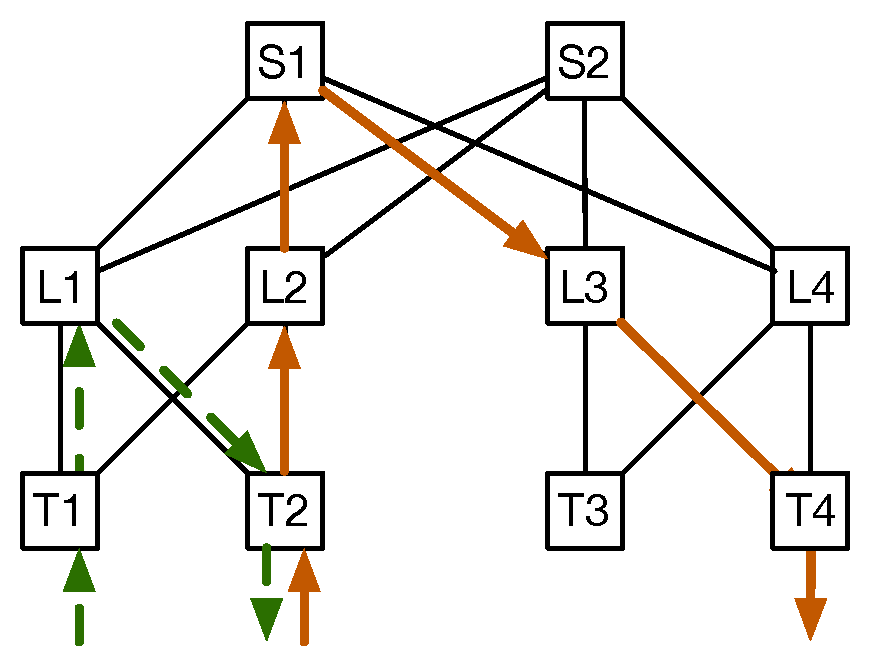
\includegraphics[width=0.4\textwidth] {figs/up-down}
	\caption{UP-DOWN routing in a Clos network.}\label{fig:up-down}
\end{figure}

Take {Figure~\ref{fig:up-down} as an example. If packets always follow the UP-DOWN routing, then deadlock cannot
happen as CBD is not possible. In up-down routing, a packet first goes UP from the source server to one of the common ancestor switches of the source and destination servers, then it goes DOWN from the common ancestor to the destination server.
In UP-DOWN routing, the following property holds: when the packet is on its way UP, it should not go DOWN; when it is on its way DOWN, it should not go UP.

However, packets may deviate from the UP-DOWN paths due to several reasons including link flapping and routing protocol flapping \cite{f10}.
As have shown in \cite{shpiner2016unlocking}, when the UP-DOWN property is broken and packets may reroute multiple times between two layers of switches, and deadlocks may form as a result.

In this paper, we show our measurement results from a large cloud computing provider that UP-DOWN routing property does break in reality and packets can be rerouted with a non negligible probability.

Our measurement works as follows. We instrument the servers to send out IP-in-IP packets to the high-layer switches. The outer source and destination IP addresses are set to the sending server and one of the high layer switches, and the inner source and destination IP addresses are set to the switch and the sending server, respectively. The high-layer switches are configured to decapsulate those IP-in-IP packets that are targeting themselves in hardware.

After decapsulation, the outer IP header is discarded, and the packet is then routed using its inner header. We set a TTL value, 64 in this paper, in the inner IP header. As the packet is forwarded back to the server, the TTL is decremented per hop. For a three-layer Clos network, there are three hops from the highest layer switches to the server. Hence normally the TTL value of the received packets should be 61.

If, however, the TTL value of a received packet is smaller than 61, say 59, we know the received packet was not taking the shortest path, and the packet must have taken a reroute path.

In this paper, for every measurement, a server sends out $n=100$ IP-in-IP probing packets, if the received TTL values are not equal, we know packet reroute happened for this measurement. We then calculate the reroute probability of the measurements as $\frac{M}{N}$, where $M$ is the number of measurements that experienced packet reroute, and $N$ is the total number of measurements. We carried out the measurements for one week in more than 20 data centers. The measurement results are shown in Table~\ref{fig:reroute}.

\begin{table}[t]
\begin{small}
\begin{center}
\begin{tabular}{|r|r|r|c|}
\hline    Date    & Total No.  & Rerouted No.   & Reroute probability \\
\hline 11/01/2016 & 11381533570 & 148416 &  1.3e-5 \\
\hline 11/02/2016 & 11056408780 & 130815 &  1.2e-5 \\
\hline 11/03/2016 & 10316034165 & 104472 &  1.0e-5 \\
\hline 11/04/2016 & 10273000622 & 92555  &  0.9e-5 \\
\hline 11/05/2016 & 10230003382 & 102872 &  1.0e-5 \\
\hline 11/06/2016 & 10491233987 & 106266 &  1.0e-5 \\
\hline 11/07/2016 & 9608289622  & 100916 &  1.1e-5 \\
\hline
\end{tabular}
\end{center}
\caption{Packet reroute measurements in the data centers of a large cloud computing service provider.}\label{fig:reroute}
\end{small}
\end{table}

The most important conclusion we can draw from Table~\ref{fig:reroute} is that packet reroute does happen in data center networks. The reroute probability is around $10^{-5}$. Though $10^{-5}$ is not a big number, given the large traffic volume and the large scale data center networks, the deadlocks due to packet reroute as discussed in \cite{rdmaatscale,shpiner2016unlocking,hu2016deadlocks} do not just exist in paper designs. They are real!

Therefore how to address potential deadlocks due to packet reroute becomes a pressing challenge.

%adding discussions on why packet reroute happen.

